%
% File acl2021.tex
%
%% Based on the style files for EMNLP 2020, which were
%% Based on the style files for ACL 2020, which were
%% Based on the style files for ACL 2018, NAACL 2018/19, which were
%% Based on the style files for ACL-2015, with some improvements
%%  taken from the NAACL-2016 style
%% Based on the style files for ACL-2014, which were, in turn,
%% based on ACL-2013, ACL-2012, ACL-2011, ACL-2010, ACL-IJCNLP-2009,
%% EACL-2009, IJCNLP-2008...
%% Based on the style files for EACL 2006 by 
%%e.agirre@ehu.es or Sergi.Balari@uab.es
%% and that of ACL 08 by Joakim Nivre and Noah Smith

\documentclass[11pt,a4paper]{article}
\usepackage[hyperref]{acl2021}
\usepackage{times}
\usepackage{latexsym}
\usepackage{amssymb}
\usepackage{amsmath}
\usepackage{graphicx}
%\usepackage{booktabs}
\renewcommand{\UrlFont}{\ttfamily\small}

% This is not strictly necessary, and may be commented out,
% but it will improve the layout of the manuscript,
% and will typically save some space.
\usepackage{microtype}

%\aclfinalcopy % Uncomment this line for the final submission
%\def\aclpaperid{***} %  Enter the acl Paper ID here

%\setlength\titlebox{5cm}
% You can expand the titlebox if you need extra space
% to show all the authors. Please do not make the titlebox
% smaller than 5cm (the original size); we will check this
% in the camera-ready version and ask you to change it back.

\newcommand\BibTeX{B\textsc{ib}\TeX}
\DeclareMathOperator*{\argmin}{arg\,min}

\title{Training Embedding Models through Direct Optimization of Clustering Goal}

\author{First Author \\
  Affiliation / Address line 1 \\
  Affiliation / Address line 2 \\
  Affiliation / Address line 3 \\
  \texttt{email@domain} \\\And
  Second Author \\
  Affiliation / Address line 1 \\
  Affiliation / Address line 2 \\
  Affiliation / Address line 3 \\
  \texttt{email@domain} \\}

\date{}

\begin{document}
\maketitle
\begin{abstract}
Existing supervised models for text clustering find it difficult to directly optimize for clustering results. This is because clustering is a discrete process and it is difficult to estimate meaningful gradient of any discrete function that can drive gradient based optimization algorithms. So, existing supervised clustering algorithms indirectly optimize for some continuous function that approximates the clustering process. We propose a training strategy that directly optimizes for a discrete clustering metric. Loss function based on this strategy is able to efficiently guide the optimization process of an embedding model towards the global clustering optima. Moreover our method is more scalable when compared to existing embedding models used for clustering. We train a BERT-based embedding model using our method and evaluate it on two publicly available datasets. We show that our method outperforms another BERT-based embedding model employing Triplet loss and other supervised and unsupervised baselines. %This suggests that optimizing directly for the clustering outcome indeed yields better embeddings suitable for clustering.
\end{abstract}

\section{Introduction}

Text clustering is a well-studied problem which finds its application in a wide range of tasks: organizing documents in cluster-based information retrieval~\cite{cutting2017scatter}~\cite{mei2014proximity}, representation of search results~\cite{37745}~\cite{navigli2010inducing}, analyzing different opinions about a subject~\cite{tsirakis2017large} among many others. Each of these applications may focus on text contents of different granularities (e.g. words, sentences, passages, articles) but all of them follow a common high-level approach to clustering: represent the documents in form of vectors and then cluster them based on vector similarities. Although clustering is typically employed in an unsupervised setting, many semi-supervised deep learning models have been proposed recently. Many of these approaches formulate this as an embedding space learning problem~\cite{yang2017towards} that projects initial document vectors into a latent vector space which is more suitable for the clustering task and generate clusters similar to some ground truth. However, most of these algorithms do not directly optimize for a clustering metric during training. Instead, they optimize for a different criterion that approximates the global clustering error. Semi-supervised clustering approaches~\cite{basu2002semi} cast the clustering problem into binary classification by learning pairwise constraints extracted from the available training examples: \textit{must-links} for sample pairs sharing the same cluster and \textit{cannot-links} for different clusters. However, for clustering problems with numerous small clusters produce only a few \textit{must-links} among all possible links, leading to highly unbalanced training data. Consequently, the trained model is biased towards predicitng \textit{cannot-links}. Learning triplet-based constraints~\cite{dor2018learning} that combine a positive and a negative sample in a single triplet, mitigate such bias towards negative samples but the sample complexity~\cite{bartlett1998sample} (number of triplet samples required to cover all interactions in a dataset) grows more rapidly compared to paired samples. Also, such approximation of the original clustering problem may lead to unsatisfactory results because the optimization criterion does not always correspond with the clustering quality. These observations motivate us to hypothesize the following:

\begin{itemize}
    \item Instead of learning to solve some approximation of the original clustering problem, we need to directly optimize for a clustering metric in order to train a model specialized for clustering.
    \item Instead of sample-pairs in case of pairwise constraints or triplets in case of Triplet-loss, we can make efficient and scalable use of the available training data by presenting all interactions between a set of data points as a single clustering sample. This way the training approach neither suffers from unbalanced data nor from sample complexity.
\end{itemize}

To test our hypotheses, we propose an alternative training strategy that directly draws its supervision signal from a clustering metric to train an embedding model for documents. During training, it consumes a complete clustering example of a set of data points as a single training sample in form of an interaction matrix.  

It is challenging to derive training signals directly from the clustering ground truth or a clustering metric because the clustering process is discrete. In other words, a function that estimates the clustering quality of a random partition of the input data is not continuous and hence non-differentiable. As most supervised algorithms rely on gradient-based optimization algorithms, it is difficult for them to orchestrate an useful training process without proper gradient. So far some continuous approximation of the clustering problem is used as discussed earlier to bypass the core optimization issue. Recently a novel gradient approximation method, \textit{blackbox backpropagation}~\cite{vlastelica2019differentiation} is proposed for combinatorial problems that finds solution in a discrete space. We leverage their findings by molding the clustering problem into a combinatorial problem. This allows us to derive meaningful gradients out of the clustering process and to train an embedding model by directly optimizing for a clustering metric.

\paragraph{Our contribution:} We make the following contributions through this work.
\begin{itemize}
    \item We develop a new training strategy for supervised clustering that directly obtains its supervision signal from optimizing a clustering metric. We utilize recently proposed \textit{blackbox backpropagation} technique to derive gradients from discrete clustering results that drives the training process.
    \item We use our training strategy to train a BERT-based embedding model suitable for topical clustering. To support the training mechanism, we design a loss function that effectively optimizes a clustering metric.
    \item We empirically show that our method is more efficient in terms of utilizing available training examples when compared to existing supervised clustering methods. The resulting embedding model achieves better clustering results than other strong baseline embedding models.
\end{itemize}


\section{Related work}
Traditionally, text clustering is achieved by employing a distance-based clustering algorithm (e.g. KMeans) on vector representations of documents (e.g. TF-IDF~\cite{jones1972statistical}). Even in recent works, authors have followed this overall approach while improving the text representation method~\cite{chen2017improved,xu2017self,hadifar2019self} or exploring different similarity metrics between the vectors that governs the clustering algorithm through pairwise binary constraints~\cite{basu2002semi,kulis2009semi}. In this work, we focus on the former - representation learning of documents, suitable for text clustering.

\textit{Deep clustering}~\cite{min2018survey} is an active field of research that aims to utilize recent advancements of deep learning techniques to improve supervised clustering. The primary focus is to learn suitable representation space that optimizes some clustering criterion (e.g. cluster assignment loss) along with a representation criterion (e.g. reconstruction loss)~\cite{xie2016unsupervised,li2018discriminatively,ghasedi2017deep,jiang2016variational}. It has also been shown that clustering criterions alone are sufficient to train such representation space~\cite{yang2016joint}. However, all these works are unsupervised in a sense that none of them attempts to receive direct supervision from a clustering ground truth. Motivated by earlier works that learn a representation model under pairwise binary constraints, Chang et al.~\cite{chang2017deep} envisions the clustering task as a binary classification task of paired data samples and achieves state-of-the-art results on multiple image clustering datasets. Reimers et al. proposes Sentence-BERT~\cite{reimers2019sentence} which trains a BERT-based~\cite{devlin2018bert} sentence embedding model by employing Triplet loss~\cite{dor2018learning} that uses triples of sentences as training samples where exactly two of them are from the same section of Wikipedia. Although both of these approaches are supervised, each training sample only consists of a fraction of the whole clustering instance and hence by no means the true representative of the clustering problem.
%While some methods take a more holistic approach of jointly optimizing for cluster assignments and representations of data samples~\cite{xie2016unsupervised}, many focus solely on learning suitable representation space.  

The main hindrance of drawing supervision signals directly from the ground truth clusters is the combinatorial nature of the problem. Some research works introduce differentiable building blocks specialized only for certain combinatorial algorithms such as satisfiability (SAT) problems~\cite{wang2019satnet}. Wilder et al.~\cite{wilder2019end} use a differentiable variant of K-means algorithm to approximate a harder combinatorial problem (graph optimization). Such relaxations of the original combinatorial problem may lead to sub-optimal results. Recently, Vlastelica et al.~\cite{vlastelica2019differentiation} proposed a novel technique of differentiating combinatorial solvers as a blackbox without any relaxation that allows us to use an optimal combinatorial algorithm as a component of a deep representation learning model and optimize it end-to-end. We give a brief background of their approach in the following section.

\subsection{\textit{Blackbox Backpropagation}}\label{sec:bb} Vlastelica et al. formalize a combinatorial solver as a mapping function between continuous input, $w \in W \subseteq \mathbb{R}^N$ and discrete output, $y \in Y$ as $w \mapsto y$ such that $y=\argmin_{y \in Y} c(w,y)$. Here $W$ is the $N$-dimensional continuous input space, $Y$ is a finite set of all possible solutions and $c$ is the cost that the solver tries to minimize. For a linear cost function $c$, they construct a continuous interpolation of the original cost function and return the gradient of this interpolation during backpropagation. The closeness of the interpolation to the original function is controlled by a single hyperparameter, $\lambda$. In our work, we extend this approach for clustering framework to draw the supervision signals directly from the clustering results and learn our model parameters.

\section{Methodology}
Our text clustering method works in two steps: 1. Train a text embedding model directly from example clusters of text snippets, 2. Cluster the trained embedding vectors using hierarchical agglomerative clustering (HAC). Our primary contribution lies in the training strategy of step 1 which we refer here as \textbf{C}lustering \textbf{O}ptimization as \textbf{B}lackbox (\textbf{COB}). We describe COB in the following sections.

\subsection{Overall approach}\label{sec:app} We envision supervised text clustering as a combinatorial problem. Let $\mathcal{P}$ be a set of $N$ documents and $Y$ be the set of all possible $k$-partitions of set $\mathcal{P}$. Also let $V_\phi$ be an embedding model with trainable parameters $\phi$. We obtain the set of representation vectors $V_\phi(\mathcal{P})$ for each of the documents in $\mathcal{P}$ using the embedding model, $V_\phi$. Based on the euclidean distances between representation vectors in $V_\phi(\mathcal{P})$, a clustering algorithm choose a particular $k$-partition $\hat{y} \in Y$ that minimizes some linear cost function $c(V_\phi(\mathcal{P}), y)$ (e.g. intra-cluster distances for HAC). Hence the clustering process can be expressed as the following mapping:
\begin{align*}
V_\phi(\mathcal{P}) \mapsto \hat{y} \quad \textrm{such that} \quad \hat{y} = \argmin_{y \in Y} c(V_\phi(\mathcal{P}), y) \\ 
\end{align*}
The clustering ground truth $y^* \in Y$ is the ideal $k$-partition of set $\mathcal{P}$. The training process of COB is governed by a loss function $\mathcal{L}(y^*,\hat{y})$ such that a clustering metric is maximized. Naturally, in order to maximize the clustering metric, $\mathcal{L}$ should be designed to inversely correlate with the clustering metric.

However, we want to emphasize here that the cost function $c(V_\phi(\mathcal{P}), y)$ is minimized as part of the clustering algorithm itself. The supervised approach we describe here, does not interfere with that. In other words, the clustering process is isolated as a \textit{blackbox} component in its entirety. The minimization of the cost function $c(V_\phi(\mathcal{P}, y)$ takes place inside this blackbox and remains opaque for our supervised model. As a result, COB is not dependent on the exact clustering algorithm we choose to implement inside the blackbox. In this work however, we choose to use HAC as our clustering algorithm. Again, we choose to optimize for RAND index in this work but our method is relevant for other clustering metrics as well (e.g. purity).

\begin{figure*}
    \centering
    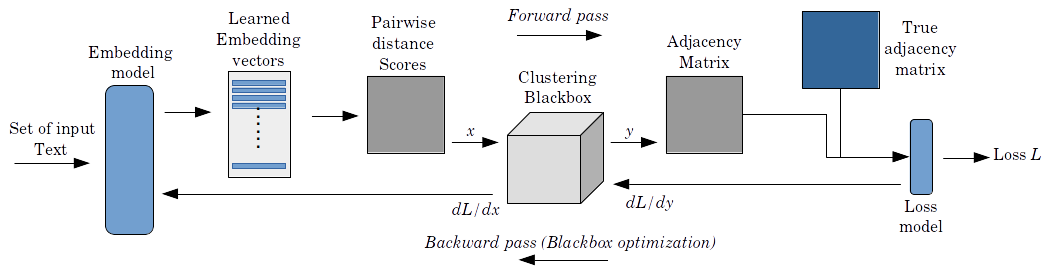
\includegraphics[scale=0.58]{acl-ijcnlp2021-templates/bbcluster_arch.png}
    \caption{Architecture of the proposed supervised clustering approach}
    \label{fig:bbc_arch}
\end{figure*}
\subsection{Optimizing for RAND index} Our goal is to train the embedding model, $V_\phi$, such that the resulting clusters maximize a clustering metric of our choice. In this work, we focus on optimizing for RAND index, a widely used clustering metric, which measures the similarity between the generated clusters and the clustering ground truth. If $y^* \in Y$ be the ground truth partition or the ideal clustering of $\mathcal{P}$, then the clustering quality of a candidate cluster $\hat{y}$ is expressed in terms of RAND index (RI):
\begin{align*}
RI &= \frac{a+b}{\binom{n}{2}}
\end{align*}
where a = sample pairs that share a cluster both in $y^*$ and $\hat{y}, b=$ sample pairs that do not share a cluster both in $y^*$ and $\hat{y}$ and $n=$ total number of data samples.

\subsection{COB Training loop}
Figure \ref{fig:bbc_arch} presents the overall training approach. The focus of the training loop is to train the embedding model $V_\phi$. First, the set of embedding vectors $V_\phi(\mathcal{P})$ is obtained for all documents in $\mathcal{P}$. Then we encode the input to the clustering algorithm as a square symmetric matrix $D$ with pairwise euclidean distance (\textit{dist}) scores between vectors in $V_\phi(\mathcal{P})$. 
%For brevity, we simply use $V$ to denote the set of all embedding vectors, $V_\phi(\mathcal{P})$, from here on.
\begin{align*}
D_{ij} = dist(V_\phi(p_i), V_\phi(p_j)) \quad \textrm{where} \quad p_i,p_j \in \mathcal{P}.    
\end{align*}
The solution to the clustering problem is expressed in form of an adjacency matrix $A$ such that
\begin{align*}
A_{ij} = 1 \textrm{ if } i,j \textrm{ share same cluster and } 0 \textrm{ otherwise}    
\end{align*}
Similarly, the clustering ground truth is expressed through another adjacency matrix, $T$. Now, we can express RI using the following form:
\begin{align*}
    RI=1-\frac{\sum |A-T|}{n^2-n} \quad \textrm{refer to Appendix}
\end{align*}
It is clear from the above equation that if we want to maximize RI, we need to minimize $\sum |A-T|$ (referred as the error matrix). Intuitively, if we are able to produce the ideal clustering results, then $A$ and $T$ would be identical, meaning $|A-T|$ is a zero matrix. Formally, we define our loss function $\mathcal{L}$ as:
\begin{align*}
\mathcal{L} = \sum_{i,j} A_{i,j}(1-T_{i,j}) + T_{i,j}(1-A_{i,j})
\end{align*}

The backward pass of this training loop involves estimating gradient of the loss $\mathcal{L}$ with respect to the distance matrix $D$, the input to the clustering black box. This is achieved using blackbox backpropagation technique and the resulting gradient is used to drive a gradient descent algorithm that eventually trains the embedding model $V_\phi$. 

\subsection{Regularization}\label{sec:reg} The purpose of any clustering algorithm is to identify groups of similar data points. By optimizing for a clustering metric such as RI, we learn the notion of similarity from a clustering ground truth. However, to capture clear distinction between similar and dissimilar data points, we need to train the embedding model in such a way that it projects similar data points close to each other and dissimilar data points far apart. This is achieved when the loss function encourages \textit{inter-cluster} distances to increase and \textit{intra-cluster} distances to decrease. Although, the HAC algorithm optimizes for similar criterion, it is separate from our training loop as we treat the clustering component as a \textit{black box}. Hence, this is incorporated into the loss function by introducing a regularizer as described below.
% If we so not include such criterion in the loss function then the model will not learn to distinguish between similar and dissimilar data enough because two clustering results may have the same ARI whether or not the similar elements are enough far apart from the dissimilar or not. But the learned model will be prone to make mistakes for unseen clustering data. Hence, it is necessary to enforce distinguishing power along with optimizing for RI.

\begin{align*}
    \mathcal{L}_{r} &= \mathcal{L} + r \cdot [\textrm{mean intra-cluster distance}\\ &- \textrm{mean inter-cluster distance}] \\
    &= \mathcal{L} + r \cdot \Bigg[\frac{\sum_{ij} D_{ij}T_{ij}}{\sum_{ij} T_{ij}} - \frac{\sum_{ij} D_{ij}(1-T_{ij})}{\sum_{ij}(1-T_{ij})}\Bigg] \\
    &\textrm{where $r$ is the regularization constant}
\end{align*}
Regularization constant $r$ controls how much emphasis we want to put on learning an accurate embedding model in terms of RI versus learning a discriminative model.

\section{Experimental results}
First, we describe the datasets used for our experiments. Next, we discuss our evaluation paradigm. Finally, we present experimental results that demonstrate efficacy of the embedding model trained using our proposed training strategy over our baseline models.

\subsection{Datasets} To evaluate our proposed approach, we use two publicly available datasets: 20 newsgroups (20NG) and TREC Complex Answer Retrieval (CAR). To compare different training strategies, we choose to evaluate them on multiple smaller clustering instances instead of a single but large clustering problem. We take the following approach to construct such clustering benchmarks from the datasets:

\subsubsection{20NG} \textbf{20NG dataset} is a widely used public collection of $18846$ documents, each categorized into any one of twenty topics. To convert this to a clustering benchmark, both train and test split of 20NG dataset is further grouped into sets of 50 documents each along with their topic labels. Each set of 50 documents represents a single instance of clustering problem. Refer to Table \ref{tab:dat20ng} for detailed statistics of the dataset.
%Random sets of 50 documents each, along with their topic labels, are extracted from train and test split. Each of these sets represent a single instance of clustering problem. 
\begin{table}[h]
\caption{Dataset statistics: $N=$ total no. of documents, $C=$ total no. of clustering instances, $d=$ average number of documents per clustering instance, $k=$ average number of clusters per clustering instance}
\begin{tabular}{llllll}
\hline
Dataset && N & C & d & k \\ \hline
20NG train && 11314 & 226 & 50 & 18 \\
20NG test  && 7532 & 150 & 50 & 18 \\ 
\end{tabular}
\label{tab:dat20ng}
\end{table}

\subsubsection{CAR} \textbf{CAR dataset} (version $2.0$ year 1) is a large collection of Wikipedia articles. Each article consists of text passages about a topic, segmented into hierarchical subtopics known as sections. From the CAR dataset, we use \texttt{train.v2.0} as train split (CAR train) and \texttt{benchmarkY1test} as test split (CAR test).  This dataset is originally designed for passage retrieval task and conveniently, passages in CAR articles are relevant for different sections under the overarching topic of the article. This relevance information is part of the dataset in form of the ground truth. So we consider each article as separate clustering problems where our task is to cluster all the passages inside it such that passages from same sections in the original article share the same cluster. We treat the section label under which a passage appears as the clustering label of the passage.

\begin{figure}[t]
    \centering
    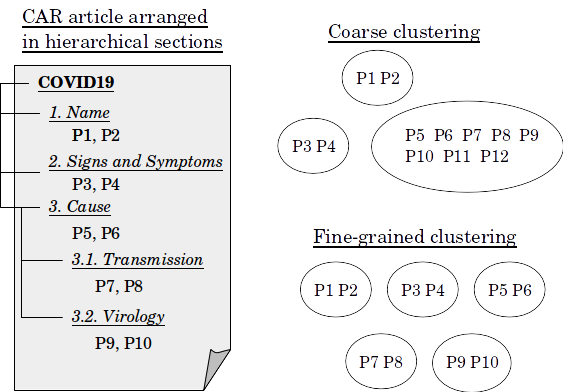
\includegraphics[scale=0.5]{acl-ijcnlp2021-templates/wiki_articles.png}
    \caption{Coarse and fine-grained clustering benchmarks from TRECCAR dataset}
    \label{fig:wiki}
\end{figure}

Section labels in TRECCAR dataset are hierarchical. This provides an opportunity to evaluate our clustering models under different levels of granularity. As depicted in Figure \ref{fig:wiki}, passages $p_6$ and $p_7$ in article \textit{COVID 19}  belong to the sections \textit{Cause} and \textit{Cause/Transmission} respectively. Under coarse view of the clustering, we will consider $p_6,p_7$ under the same topic cluster \textit{Cause}. However, for fine-grained clustering we have to consider $p_6,p_7$ under separate subtopic clusters. Fortunately, TRECCAR dataset provides both in form of \textit{top-level} (coarse) and \textit{hierarchical} (fine-grained) benchmarks. We train and evaluate our models on both flavors of the dataset. Statistics of the datasets are provided in Table \ref{tab:dat}.

%need to find out best way to represent stats of dataset
\begin{table}[h]
\caption{Dataset statistics: $N,C,d,k$ denotes the same as Table \ref{tab:dat20ng}. Here, each clustering instance is a set of passages relevant for an article in Wikipedia.}
\begin{tabular}{llllll}
\hline
Dataset & N & C & d & $k_{coarse}$ & $k_{fine}$ \\ \hline
CAR train  & 6.8M & 597K & 11 & 3.84 & 5.04 \\
CAR test   & 6K & 126 & 47 & 7.78 & 17.16   
\end{tabular}
\label{tab:dat}
\end{table}

\subsection{Evaluation paradigm} Our primary focus is to evaluate the efficacy of our proposed training strategy for supervised clustering and compare it with other training methods while ensuring the fairness of our evaluation. Hence, we train the same embedding model with the same training data differing only in the training strategies. Finally, average performance on all clustering instances in the test splits are reported with statistical significance testing. 

\subsubsection{Baseline methods:} In order to conduct a thorough comparative study, we include the following baseline methods into our evaluation:

\textbf{SBERT-Triplet:} To compare our approach with a strong supervised baseline, we use Sentence-BERT~\cite{reimers2019sentence}, a recent BERT-based embedding model retrained on our dataset. They employ Triplet loss~\cite{dor2018learning}, specifically designed to generate embeddings suitable for text clustering. Here, each training sample consists of two similar ($a,p$) and one dissimilar ($n$) embedding vectors. Triplet loss trains the embedding model so that the distance between $a,p$ is less than $a,n$ by at least a margin $\epsilon$.

\begin{align*}
    \mathcal{L}_{triplet} = max(||a-p||-||a-n||+\epsilon, 0)
\end{align*}

%\textbf{SBERT Binary} Similar to SBERT-Triplet except the Triplet loss is replaced by Binary loss. Inspired from works in image clustering~\cite{chang2017deep}, Binary loss simplifies the clustering process as a binary classification problem where each training sample consists of a pair of similar or dissimilar data points.

\textbf{Unsupervised baselines:} We also include \textbf{DBC} (Discriminatively Boosted Clustering), a recent deep unsupervised clustering approach proposed by Li et al.~\cite{li2018discriminatively} and \textbf{TFIDF} with cosine similarity (as a more canonical approach) to compare the performances of unsupervised clustering approaches for our use cases.

We use Adjusted RAND index (ARI) and Normalized Mutual Information (NMI) as our clustering evaluation metric.

\subsection{Clustering evaluation} Here we present details of all the experiments carried out and discuss the results. All experiments are executed in a GPU server hosting a single NVIDIA Titan XP GPU with around 12GB memory.

\subsubsection{Experiment 1: 20NG} We train COB and other supervised methods using the train split of 20NG dataset with around $20\%$ held out for validation. All methods are trained until no significant improvement on validation performance is observed. For each method, we use the best model found during training in terms of validation performance to evaluate on the test set. Table \ref{tab:ng20exp} presents the performance on test sets evaluated using mean ARI and NMI.

\begin{table}[h]
\caption{Clustering performance on NG20 dataset in terms of mean Adjusted RAND Index (ARI) and mean Normalized Mutual Information (NMI). Paired ttest ($\alpha=0.05$) is carried out with respect to SBERT Triplet and $\blacktriangle$ and $\blacktriangledown$ denotes significantly higher or lower performance.}
\label{tab:ng20exp}
\begin{tabular}{lll}
\hline
Method        & mean ARI & mean NMI \\ \hline
TFIDF         & 0.008$\blacktriangledown$ & 0.506$\blacktriangledown$ \\
DBC           & 0.042$\blacktriangledown$ & 0.584$\blacktriangledown$ \\
%SBERT Binary  &          &          \\
SBERT Triplet & 0.223 & 0.721 \\
SBERT COB     & \textbf{0.233}$\blacktriangle$ & \textbf{0.725}$\blacktriangle$        
\end{tabular}
\end{table}

As we observe from Table \ref{tab:ng20exp}, our proposed method SBERT COB outperforms all other baselines in terms of ARI and NMI. The improvement is statistically significant in terms of paired ttest carried out with respect to the best performing baseline, SBERT Triplet. Both TFIDF and DBC fail to obtain meaningful clusters, suggesting the efficacy of supervised embedding models in clustering context.

\subsubsection{Experiment 2: CAR} Due to large size of the CAR training split (\texttt{train.v2.0}), it is impractical to train \textbf{SBERT Triplet} with all possible triplets in the training set. Instead, we compare the supervised models trained on three smaller splits of the training dataset. Each split contains articles that has exactly $n$ passages where $n=30, 35$ and $40$. Table \ref{tab:datsplit} has statistics about these three training splits. 

\begin{table}[h]
\caption{Dataset statistics: $n=$ total no. of passages in each article in this split}
\label{tab:datsplit}
\begin{tabular}{lllll}
\hline
\multicolumn{1}{c}{Splits} & \multicolumn{1}{c}{Articles} & \multicolumn{1}{c}{Passages} & \multicolumn{2}{c}{Triplets}                                  \\
\multicolumn{1}{c}{}       & \multicolumn{1}{c}{}         & \multicolumn{1}{c}{}         & \multicolumn{1}{c}{Coarse} & \multicolumn{1}{c}{Fine} \\ \hline
n=30 & 2376 & 71280 & 8.6M & 5.8M \\
n=35 & 1605 & 56175 & 9.3M & 5.9M \\
n=40 & 1248 & 49920 & 10.8M & 6.5M                                
\end{tabular}
\end{table}

\begin{table}[h]
\caption{Coarse-level clustering performance on TRECCAR dataset using top-level benchmarks. Supervised models are trained with set of clustering examples each containing $n$ passages. Paired ttest ($\alpha=0.05$) is carried out with respect to SBERT Triplet ($n=30$).}
\label{tab:trecexp}
\begin{tabular}{lll}
\hline
Method        & mean ARI & mean NMI \\ \hline
TFIDF         & 0.072$\blacktriangledown$ & 0.375$\blacktriangledown$ \\ \hline
%SBERT Binary  &          &          \\
n=30&&\\
DBC           & 0.075$\blacktriangledown$ & 0.375$\blacktriangledown$ \\ 
%SBERT Triplet & 0.192 & 0.478 \\
SBERT Triplet & 0.214 & 0.494 \\
SBERT COB     & 0.230 & 0.502 \\ \hline
n=35&&\\
DBC           & 0.069$\blacktriangledown$ & 0.367$\blacktriangledown$ \\ 
SBERT Triplet & 0.167$\blacktriangledown$ & 0.460$\blacktriangledown$ \\
SBERT COB     & \textbf{0.236} & 0.512$\blacktriangle$ \\ \hline
n=40&&\\
DBC           & 0.036$\blacktriangledown$ & 0.330$\blacktriangledown$ \\ 
SBERT Triplet & 0.145$\blacktriangledown$ & 0.438$\blacktriangledown$ \\
SBERT COB     & 0.231 & \textbf{0.514}$\blacktriangle$  
\end{tabular}
\end{table}

\begin{table}[h]
\caption{Fine-grained clustering performance on TRECCAR dataset using hierarchical benchmarks. Notations used are similar to that in Table \ref{tab:trecexp}}
\label{tab:trecexp2}
\begin{tabular}{lll}
\hline
Method        & mean ARI & mean NMI \\ \hline
TFIDF         & 0.110$\blacktriangledown$ & 0.631$\blacktriangledown$ \\ \hline
%SBERT Binary  &          &          \\
n=30&&\\
DBC           & 0.089$\blacktriangledown$ & 0.607$\blacktriangledown$ \\
%SBERT Triplet & 0.162 & 0.673 \\
SBERT Triplet & 0.173 & 0.678 \\
SBERT COB     & \textbf{0.178} & \textbf{0.682} \\ \hline
n=35&&\\
DBC           & 0.077$\blacktriangledown$ & 0.595$\blacktriangledown$ \\
%SBERT Triplet & 0.167 & 0.675 \\
SBERT Triplet & 0.152$\blacktriangledown$ & 0.665$\blacktriangledown$ \\
SBERT COB     & 0.163 & 0.672 \\ \hline
n=40&&\\
DBC           & 0.066$\blacktriangledown$ & 0.582$\blacktriangledown$ \\
%SBERT Triplet & 0.110$\blacktriangledown$ & 0.646$\blacktriangledown$ \\
SBERT Triplet & & \\
SBERT COB     & 0.154 & 0.666$\blacktriangledown$
\end{tabular}
\end{table}

We report the coarse and fine-grained clustering performance in Table \ref{tab:trecexp} and Table \ref{tab:trecexp2} respectively. For coarse clustering, we observe that for every training splits ($n=30,35,40$) our proposed method SBERT COB performs significantly better than the best performing baseline, SBERT Triplet ($n=30$) in terms of both ARI and NMI. In case of fine-grained clustering, SBERT COB still achieves better or on par clustering performance in terms of ARI over SBERT Triplet although the differences are not statistically significant. This is expected as fine-grained clustering is a harder clustering problem largely due to less number of passage pairs sharing a cluster. Note that NMI measures are only comparable within a Table because unlike ARI it is not adjusted for chance.

\subsection{Training convergence} 
\begin{figure*}[t]
    \centering
    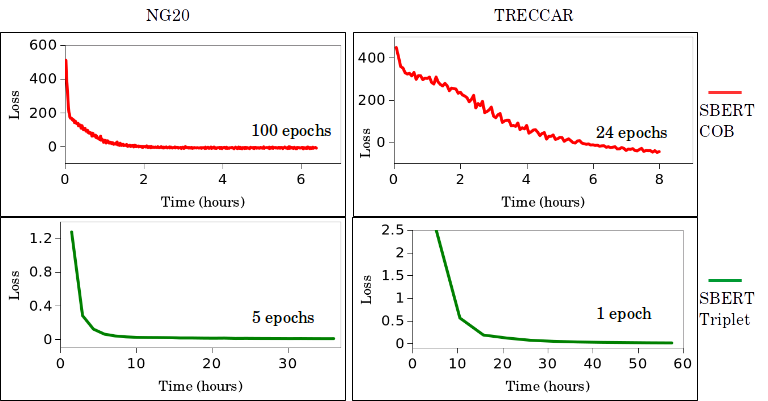
\includegraphics[scale=0.75]{acl-ijcnlp2021-templates/training_loss.png}
    \caption{Training convergence}
    \label{fig:train}
\end{figure*}

The key difference between existing training strategies for supervised clustering and COB is that it incorporates an entire clustering instance into a single training sample. This allows the model to learn the complex interactions between all data samples in a holistic fashion and train the embedding mechanism accordingly. This is particularly helpful when we want to optimize a clustering metric as in our case. 
\begin{figure*}[h]
    \centering
    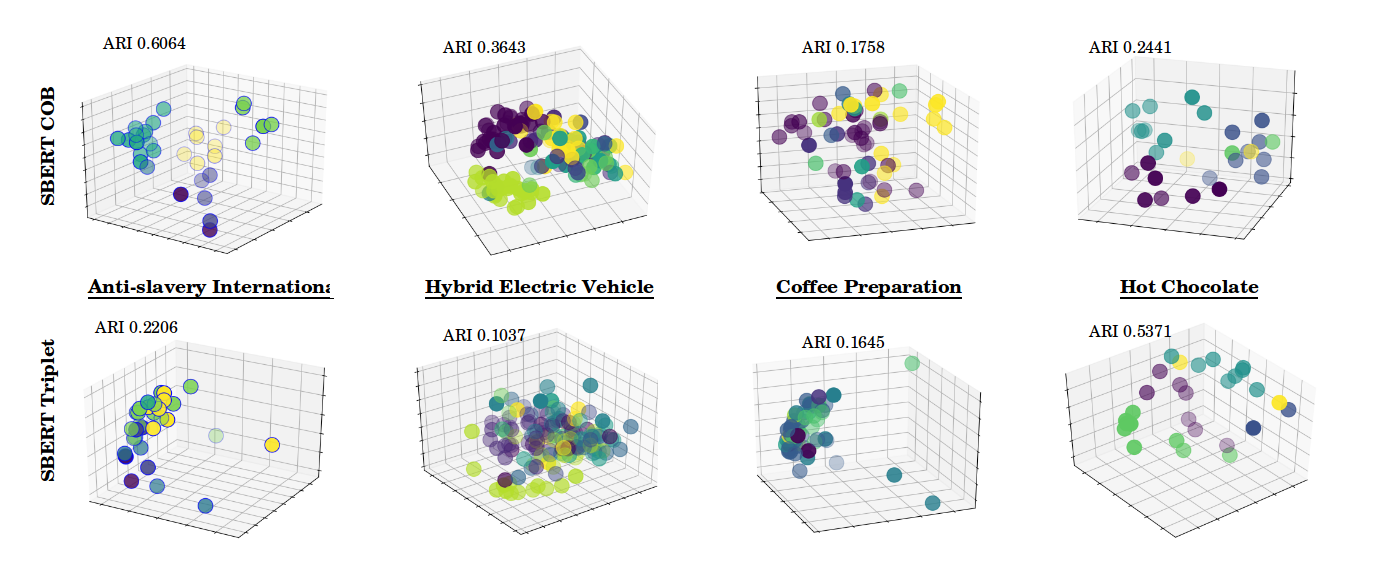
\includegraphics[scale=0.45]{acl-ijcnlp2021-templates/compare_cluster_viz.png}
    \caption{Visual comparison of clustering results}
    \label{fig:viz}
\end{figure*}

To demonstrate this we present Figure \ref{fig:train} that depicts the training progress of SBERT Triplet and SBERT COB on 20NG dataset and TRECCAR dataset (coarse $n=35$) respectively. For 20NG dataset, we observe that SBERT Triplet converges only after three iterations over all the triplets in the dataset. However, SBERT COB takes around $40$ iterations to converge but achieves better clustering performance according to validation ARI. As SBERT Triplet is agnostic to the overall clustering performance of the trained model, it converges quickly after optimizing a relaxed version of the clustering problem, the triplet loss. But SBERT COB has a more complex loss landscape to explore that results in slow convergence in terms of number of iterations but allows it to learn more accurate representation of the clustering solution. Here we want to also emphasize that a single iteration of SBERT COB is much faster than the same of SBERT Triplet as reported in figure. Due to this, SBERT COB is able to reach convergence much faster than SBERT Triplet in terms of time in hours. We observe similar results on TRECCAR dataset.

\subsection{Overfitting on TRECCAR dataset} Unlike NG20, we observe that both the models suffer from overfitting according to the validation performance on both flavors of the TRECCAR dataset. Note here that each clustering instance in NG20 is a sample of documents drawn from the same distribution of twenty topics. But for TRECCAR, each clustering instance is a set of passages relevant for a specific topic in Wikipedia. This is why it is difficult to learn a generalized clustering model for TRECCAR dataset. Despite the fact, SBERT COB is able to consistently achieve high ARI scores on the test set as demonstrated earlier suggesting that SBERT COB is able to generalize better than SBERT Triplet.

\subsection{Hyperparameter optimization} SBERT COB has a pair of hyperparameters, interpolation parameter $\lambda$ (refer to Section \ref{sec:bb}) and regularization constant $r$ (refer to Section \ref{sec:reg}). We use Optuna~\cite{optuna_2019}, a recently proposed hyperparameter optimization framework, to search for optimum $\lambda, r$ pair in terms of validation performance for each dataset.

\subsection{Qualitative evaluation} Here, we demonstrate efficacy of SBERT COB over SBERT Triplet ($n=35$) through visual comparison of some clustering results from the TRECCAR dataset. Principle Component Analysis (PCA) is used to transform the embedding vectors into 3D vectors which are then visualized as points in 3D vector space. Figure \ref{fig:viz} compares the results obtained for four articles from TRECCAR test split.

As we can observe, for articles \textit{Anti-slavery International} and \textit{Hybrid Electric Vehicle}, SBERT COB is able to clearly identify clusters of different topics and projects them in different regions of the embedding space. On the contrary, it is difficult to find any clear cluster boundaries in the SBERT Triplet embedding space and it reflects in the ARI scores obtained by the methods. For the article \textit{Coffee Preparation}, although in terms of ARI scores both the methods perform poorly, at least in case of SBERT COB we see tendency to separate dissimilar passages. SBERT Triplet projects almost all the passages in a dense region except for a few outlier passages. For the article \textit{Hot Chocolate}, SBERT Triplet obtains numerous small clusters of similar passages. As ARI metric is pair-based, SBERT Triplet obtains better ARI score even though it does not achieve clear groupings of similar elements.

It is clear from the examples that SBERT COB has a better sense of global clustering quality than SBERT Triplet. This is expected because unlike SBERT Triplet, SBERT COB observes the relationships between all data samples of a clustering instance at once and using that learns to directly optimize for a clustering metric. %Although sometimes it fools ARI, but visually SBERT COB is better

\section{Conclusion} In this work, we propose an alternative training strategy to train an embedding model, suitable for clustering. Our training strategy, COB (Clustering Optimization as Blackbox), directly optimizes RAND index, a clustering metric. Using COB, we train SBERT COB, a BERT-based text representation model. We empirically show that SBERT COB significantly outperforms other supervised and unsupervised text embedding model on two separate datasets in terms of ARI and NMI, indicating better cluster quality. Visual representations of the embeddings also confirm that SBERT COB learns to holistically distinguish separate clusters from a set of text passages. Moreover, each epoch in SBERT COB training loop takes only a fraction of time when compared to SBERT Triplet, our best performing baseline method. This leads to significant decrease in overall training time. Also, compared to Triplet-based training method, SBERT COB is able to make efficient use of available training samples.

\bibliographystyle{acl_natbib}
\bibliography{acl2021}

%\appendix



\end{document}
